
\documentclass[letterpaper, reqno,11pt]{article}
\usepackage[margin=1.0in]{geometry}
\usepackage{color,latexsym,amsmath,amssymb}
\usepackage{fancyhdr}
\usepackage{amsthm}
\usepackage{mathtools}
\usepackage{tikz}
\usepackage{float}
\usepackage{centernot}
\usepackage{subcaption}
\usepackage{extarrows}
\usetikzlibrary{hobby}
\usetikzlibrary{shapes.multipart}
\usepackage{pgfplots}
\pgfplotsset{compat=1.7}
\usetikzlibrary{arrows.meta}
\usepackage{cancel}
\usetikzlibrary{decorations.markings}
\usetikzlibrary{shapes}

\newcommand{\RR}{\mathbb{R}}
\newcommand{\CC}{\mathbb{C}}
\newcommand{\ZZ}{\mathbb{Z}}
\newcommand{\QQ}{\mathbb{Q}}
\newcommand{\NN}{\mathbb{N}}
\def\upint{\mathchoice%
  {\mkern13mu\overline{\vphantom{\intop}\mkern7mu}\mkern-20mu}%
  {\mkern7mu\overline{\vphantom{\intop}\mkern7mu}\mkern-14mu}%
  {\mkern7mu\overline{\vphantom{\intop}\mkern7mu}\mkern-14mu}%
  {\mkern7mu\overline{\vphantom{\intop}\mkern7mu}\mkern-14mu}%
  \int}
\def\lowint{\mkern3mu\underline{\vphantom{\intop}\mkern7mu}\mkern-10mu\int}
\DeclareMathOperator{\card}{card}
\DeclareMathOperator{\Binomial}{Binomial}
\DeclareMathOperator{\Span}{span}
\pagestyle{fancy}
\lhead{Math 321 Lecture 23}
\rhead{Yuchong Pan}
\begin{document}
\pagenumbering{arabic}
\title{Math 321 Lecture 23}
\author{Yuchong Pan}
\date{March 4, 2019}
\newtheorem{thm}{Theorem}
\newtheorem{defn}{Definition}
\newtheorem*{remark}{Remark}
\newtheorem{claim}{Claim}
\newtheorem{cor}{Corollary}
\newtheorem{lemma}{Lemma}
\newtheorem{prop}{Proposition}
\newtheorem{fact}{Fact}
\maketitle
%

\section{Fourier Series (Cont'd)}

Let $f \in \mathcal C^{2\pi}$. Last time we saw that $s_n f = \text{$n^\text{th}$ partial Fourier sum of $f$}$ is a ``distance-minimizer'' in the following sum:
\[ \lVert f - s_n f \rVert_2 = \min \{ \lVert f - T \rVert_2 : T \in V_n \}, \qquad V_n = \Span \{ 1, \cos kx, \sin kx : 1 \leq k \leq n \}. \]

\begin{figure}[H]
  \centering
  \begin{tikzpicture}
    \draw (0, 0) -- (10, 0) node [right] {$V_n$};
    \draw[red, thick] (5, 0) -- (5, 2.5);
    \draw (5, 2.5) -- (1.5, 0) node[below] {$T$};
    \draw (5, 2.5) -- (3, 0) node[below] {$T$};
    \draw (5, 2.5) -- (6.5, 0) node[below] {$T$};
    \node[below] at (5, 0) {$s_n f$};
    \node[right] at (5, 2.5) {$f \in L_*^2$};
  \end{tikzpicture}
\end{figure}

We showed
\begin{equation} \label{eq:*} \tag{*}
  \fbox{\text{$\lVert f \rVert_2^2 = \lVert s_n f \rVert_2^2 + \lVert f - s_n f \rVert_2^2$.}}
\end{equation}

\begin{figure}[H]
  \centering
  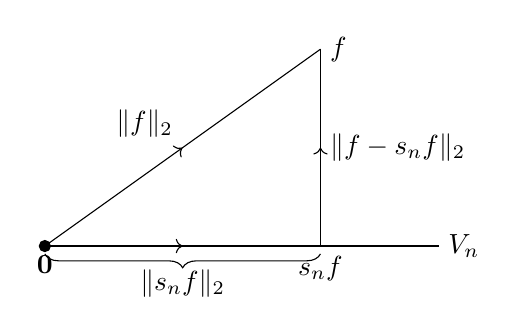
\begin{tikzpicture}
    \draw (0, 0) -- (5, 0) node [right] {$V_n$};
    \draw[decoration={
        markings,
        mark=at position 0.5 with {\arrow{>}}},
      postaction={decorate}
    ] (0, 0) -- (3.5, 0) node [below] {$s_n f$};
    \draw[decoration={
        markings,
        mark=at position 0.5 with {\arrow{>}}},
      postaction={decorate}
    ] (3.5, 0) -- (3.5, 2.5) node[midway, right] {$\lVert f - s_n f \rVert_2$};
    \draw[decoration={
        markings,
        mark=at position 0.5 with {\arrow{>}}},
      postaction={decorate}
    ] (0, 0) -- (3.5, 2.5) node[midway, above left] {$\lVert f \rVert_2$};
    \draw[fill=black] (0, 0) circle (2pt) node [below] {$\mathbf 0$};
    \node[right] at (3.5, 2.5) {$f$};
    \draw[decoration={brace, raise=0.1cm, amplitude=5pt}, decorate] (3.5, 0) -- (0, 0) node [midway, below, yshift=-5pt] {$\lVert s_n f \rVert_2$};
  \end{tikzpicture}
\end{figure}

We have
\begin{align*}
  \eqref{eq:*} \Rightarrow \lVert s_n f \rVert_2^2 &\leq \lVert s_n f \rVert_2^2 + \lVert f - s_n f \rVert_2^2 \\
  &= \lVert f \rVert_2^2. && \text{by \eqref{eq:*}}
\end{align*}

Recall: $s_n f(x) = \alpha_0 + \sum_{k = 1}^n (\alpha_k \cos kx + \beta_k \sin kx)$. Therefore,
\[ \lVert s_n f \rVert_2^2 = \frac{1}{2\pi} \int_{-\pi}^\pi |s_n f(x)|^2 dx = \underbrace{\alpha_0^2 + \frac{1}{2} \sum_{k = 1}^n \left(\alpha_k^2 + \beta_k^2\right)^2}_\text{checked last time}. \]
Get
\[ \fbox{\text{$\underbrace{\alpha_0^2 + \frac{1}{2} \sum_{k = 1}^n \left(\alpha_k^2 + \beta_k^2\right)}_\text{depend on $n$ and increases with $n$} \leq \underbrace{\lVert f \rVert_2^2}_\text{independent of $n$}$}} \text{ : Bassel's inequality.} \]
Let $n \nearrow \infty$ to get: $\alpha_0^2 + \frac{1}{2} \sum_{k = 1}^n \left(\alpha_k^2 + \beta_k^2\right)$ is convergent sum, whose value is $\leq \lVert f \rVert_2^2$.

\begin{thm}[Plancherel]
  \normalfont For every $\underbrace{f \in \mathcal C^{2\pi}}_\text{$\leadsto$ $f$ Riemann integrable ($\alpha(x) = x$) [Exercise]}$,
  \begin{enumerate}
  \item $\lVert f - s_n f \rVert_2 \xrightarrow{\text{as $n \to \infty$}} 0$.

    (In other words, $s_n f$ provides a good approximation of $f$ in the sense of $L_*^2$.)
  \item $\alpha_0^2 + \frac{1}{2} \sum_{k = 1}^\infty \left(\alpha_k^2 + \beta_k^2\right) = \lVert f \rVert_2^2$ (Parseval identity).

    Say that $\{ c_1 , c_k \cos kx, d_k \sin kx : k \geq 1 \}$ is an ``\emph{orthonormal}'' basis of $L_*^2$.
  \end{enumerate}
\end{thm}

\noindent {\bf Example from linear algebra:}

\medskip

$\RR^2, \mathbf v \in \RR^2, \mathbf v = \begin{pmatrix} v_1 \\ v_2 \end{pmatrix} = \alpha_1 \mathbf w_1 + \alpha_2 \mathbf w_2$ with $\lVert \mathbf v \rVert^2 = \alpha_1^2 + \alpha_2^2$ \emph{provided} $\{ \mathbf w_1, \mathbf w_2 \}$ is an \fbox{orthonormal} basis of $\RR^2$.

\[ \mathbf v = \fbox{$v_1$} \underbrace{\begin{pmatrix} 1 \\ 0 \end{pmatrix}}_{= \mathbf e_1} + \fbox{$v_2$} \underbrace{\begin{pmatrix} 0 \\ 1 \end{pmatrix}}_{= \mathbf e_2} = \underbrace{\fbox{$\frac{v_1 + v_2}{2}$}}_{= a_1} \underbrace{\frac{1}{\sqrt 2} \begin{pmatrix} 1 \\ 1 \end{pmatrix}}_{= \mathbf f_1} + \underbrace{\fbox{$\frac{v_1 - v_2}{2}$}}_{= a_2} \underbrace{\frac{1}{\sqrt 2} \begin{pmatrix} 1 \\ -1 \end{pmatrix}}_{= \mathbf f_2} = \fbox{$b_1$} \begin{pmatrix} 1 \\ 0 \end{pmatrix} + \fbox{$b_2$} \begin{pmatrix} 1 \\ 1 \end{pmatrix}. \]
Then,
\[ \lVert \mathbf v \rVert = v_1^2 + v_2^2 = a_1^2 + a_2^2 \neq b_1^2 + b_2^2. \]

\begin{proof}[Proof of Plancherel's theorem]
  \begin{enumerate}
  \item \label{enum:1} Take any $T \in V_n = \Span\{ 1, \cos kx, \sin kx : 1 \leq k \leq n \}$.
    \begin{align*}
      & \lVert f - T \rVert_2^2 = \frac{1}{2\pi} \underbrace{|f(x) - T(x)|^2}_{\leq \lVert f - T \rVert_\infty^2} dx && \lVert f - T \rVert_\infty = \sup_{x \in [-\pi, \pi]} |f(x) - T(x)| \\
      \Rightarrow ~ & \lVert f - T \rVert_2 \leq \lVert f - T \rVert_\infty \\
      \Rightarrow ~ & \underbrace{\inf \{ \lVert f - T \rVert_2 : T \in V_n \}}_{ = \lVert f - s_n f \rVert_2} \leq \underbrace{\inf \{ \lVert f - T \rVert_\infty : T \in V_n \xrightarrow{n \to \infty} 0}_{\substack{\text{this is true by Weierstrass's second theorem} \\ \text{(there exists a trignometric polynomial $P_n$} \\ \text{such that $\lVert P_n - f \rVert_\infty \xrightarrow{n \to \infty} 0$)}}}.
    \end{align*}
  \item If $\lVert s_n f - f \rVert_2 \xrightarrow{n \to \infty} 0$ (know this by part \ref{enum:1}), we have
    \[ \lim_{n \to \infty} \lVert s_n f \rVert_2 = \lVert f \rVert_2, \]
    because $| \lVert s_n f \rVert_2 - \lVert f \rVert_2| \leq \lVert s_n f - f \rVert_2$ by the triangular inequality. We need to show
    \begin{align*}
      \lVert s_n f \rVert_2 - \lVert f \rVert_2 &\leq \lVert s_n f - f \rVert_2, \\
      \lVert f \rVert_2 - \lVert s_n f \rVert_2 &\leq \lVert s_n f - f \rVert_2.
    \end{align*}
    Therefore,
    \[ \lim_{n \to \infty} \lVert s_n f \rVert_2 = \lVert f \rVert_2 \Rightarrow \lim_{n \to \infty} \lVert s_n f \rVert_2^2 = \lVert f \rVert_2^2 \Rightarrow \lim_{n \to \infty} \left[\alpha_0^2 + \frac{1}{2} \sum_{k = 1}^n \left(\alpha_k^2 + \beta_k^2\right)\right] = \lVert f \rVert_2^2. \]
  \end{enumerate}
\end{proof}

\noindent {\bf $L^2$-primer:}

\begin{figure}[H]
  \centering
  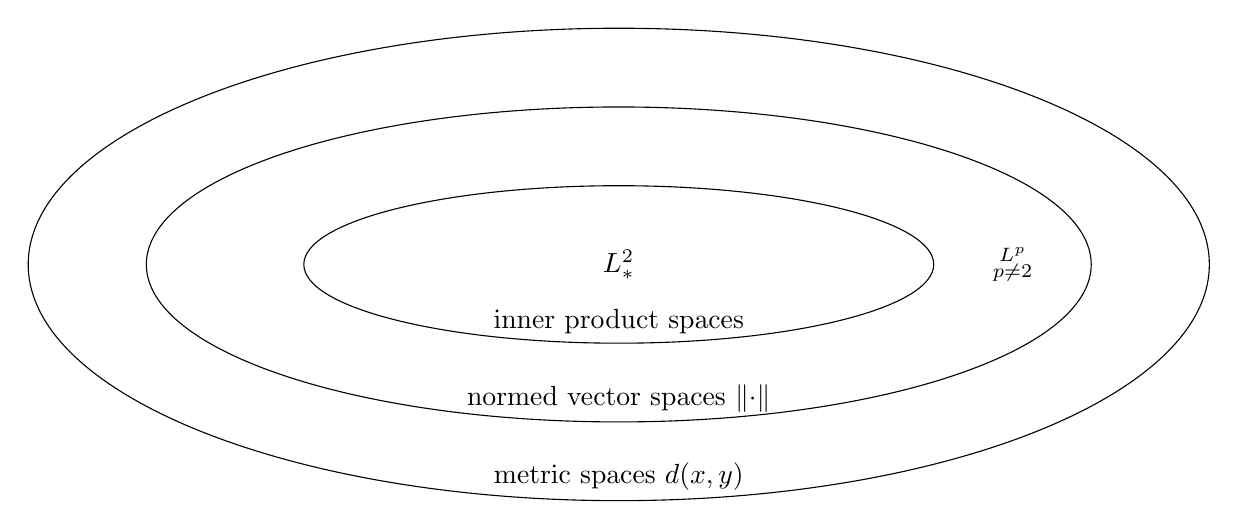
\begin{tikzpicture}
    \draw (0, 0) ellipse (7.5 and 3);
    \node[above] at (0, -3) {metric spaces $d(x, y)$};
    \draw (0, 0) ellipse (6 and 2);
    \node[above] at (0, -2) {normed vector spaces $\lVert \cdot \rVert$};
    \node at (5, 0) {$\substack{L^p \\ p \neq 2}$};
    \draw (0, 0) ellipse (4 and 1) node {$L_*^2$};
    \node[above] at (0, -1) {inner product spaces};
  \end{tikzpicture}
\end{figure}

\begin{defn}
  \normalfont Let $f, g \in L_*^2$. Define
  \[ \langle f, g \rangle = \frac{1}{2\pi} \int_{-\pi}^\pi f(x) g(x) dx. \]
\end{defn}

\end{document}
